%; whizzy chapter
% -initex iniptex -latex platex -format platex -bibtex jbibtex -fmt fmt
% 以上 whizzytex を使用する場合の設定。


%     Tokyo Debian Meeting resources
%     Copyright (C) 2006 Junichi Uekawa

%     This program is free software; you can redistribute it and/or modify
%     it under the terms of the GNU General Public License as published by
%     the Free Software Foundation; either version 2 of the License, or
%     (at your option) any later version.

%     This program is distributed in the hope that it will be useful,
%     but WITHOUT ANY WARRANTY; without even the implied warranty of
%     MERCHANTABILITY or FITNESS FOR A PARTICULAR PURPOSE.  See the
%     GNU General Public License for more details.

%     You should have received a copy of the GNU General Public License
%     along with this program; if not, write to the Free Software
%     Foundation, Inc., 51 Franklin St, Fifth Floor, Boston, MA  02110-1301 USA

%   Pdf作成手順
% dvipdfmx debianmeetingresume200609.dvi
%  preview (shell-command (concat "xpdf " (replace-regexp-in-string "tex$" "pdf"(buffer-file-name)) "&"))
% 画像ファイルを処理するためにはebbを利用してboundingboxを作成。
%(shell-command "cd image200609; ebb *.png")

%%ここからヘッダ開始。

\documentclass[mingoth,a4paper]{jsarticle}
\usepackage[dvipdfmx]{graphicx}
\usepackage{fancybox}
\usepackage{longtable}
\usepackage{ascmac}	% 囲み (screen,itembox)
\usepackage{fancyvrb}   % 囲み Verbatim のために必要
\usepackage[dvipdfmx]{hyperref}
\usepackage{url}
\usepackage[dvipdfmx]{color}

%http://www.naney.org/diki/dk/hyperref.html
%日本語EUC系環境の時
\AtBeginDvi{\special{pdf:tounicode EUC-UCS2}}
%シフトJIS系環境の時
%\AtBeginDvi{\special{pdf:tounicode 90ms-RKSJ-UCS2}}

%% spacing の設定をする。外枠を減らす。
\setlength\headheight{0mm}
\setlength\topmargin{-20mm}
\setlength\headsep{0mm}
\setlength\topskip{3mm}
\setlength\maxdepth{4pt}
\setlength\columnsep{6mm}
\setlength\textheight{252mm}
\setlength\topmargin{-5mm}
\setlength\textwidth{170mm}
\setlength\oddsidemargin{-5mm}
\setlength\evensidemargin{-5mm}

% commandline環境を定義。画面入出力についてはcommandline環境
% で表記する
\newenvironment{commandline}%
{\VerbatimEnvironment
  \begin{Sbox}\begin{minipage}{15cm}\begin{fontsize}{7.3}{7.3} \begin{BVerbatim}}%
{\end{BVerbatim}\end{fontsize}\end{minipage}\end{Sbox}
  \setlength{\fboxsep}{8pt}\fbox{\TheSbox}}


%%% start of santaku
\makeatletter
\newwrite\tf@jqz
\immediate\openout\tf@jqz\jobname.jqz\relax
\makeatother
\newcounter{santakucounter}
\newcommand{\santaku}[5]{%
\addtocounter{santakucounter}{1}

\addtocontents{jqz}{\arabic{santakucounter}. #5\\}
\begin{minipage}{1\hsize}
問題\arabic{santakucounter}. 
#1\\
□ A #2\\
□ B #3\\
□ C #4
\end{minipage}
\hspace{1cm}
\\

}
%%% end of santaku

\newcommand{\emptyspace}{(\underline{\hspace{1cm}})}

\newcommand{\subsubsubsection}[1]{%
\vspace{1zw}{\bf #1}\\}


% sectionをセンタリングする
\makeatletter
  \renewcommand{\section}{\@startsection{section}{1}{\z@}%
    {\Cvs \@plus.5\Cdp \@minus.2\Cdp}% 前アキ
    {.5\Cvs \@plus.3\Cdp}% 後アキ
    {\normalfont\Huge\headfont\raggedright\centering}} % style
\makeatother

% section の代わりの環境
\newcommand{\dancersection}[2]{%
\newpage
東京エリアDebian勉強会 2006
\hrule
\vspace{0.5mm}
\hrule
%\hfill{}
\includegraphics[width=3cm]{image200502/openlogo-nd.eps}\\
\hfill{}
\includegraphics[width=16cm]{image2006-natsu/guruguru-sand-light.png}\\
\vspace{-5cm}
\begin{center}
\section{#1}
\end{center}
\hfill{}\colorbox{white}{#2}\hspace{3cm}\space\\
\vspace{1cm}
\hrule
\vspace{0.5mm}
\hrule
\vspace{1cm}
}

% BTSの番号を見るためのコマンド
\newcommand{\debianbug}[1]{#1\footnote{\url{http://bugs.debian.org/#1}}}

% for dancerj
\newcommand{\fgref}[1]{図\ref{#1}}
\newcommand{\tbref}[1]{表\ref{#1}}


\begin{document}

\begin{titlepage}

% 毎月変更する部分, 本文の末尾も修正することをわすれずに
\title{
 第20回 東京エリア Debian 勉強会\\事前資料}
\date{2006年9月16日}
\author{Debian勉強会会場係 上川 純一\thanks{Debian Project Official Developer}} 
\maketitle
\thispagestyle{empty}
\end{titlepage}

\newpage
\tableofcontents

\dancersection{Introduction To Debian 勉強会}{上川 純一}

今月のDebian勉強会へようこそ。
これからDebianのあやしい世界に入るという方も、すでにどっぷりとつかってい
るという方も、月に一回Debianについて語りませんか?

目的として下記の二つを考えています。

\begin{itemize}
 \item メールではよみとれない、もしくはよみとってられないような情報を情
       報共有する場をつくる
 \item まとまっていないDebianを利用する際の情報をまとめて、ある程度の塊と
       して出してみる
\end{itemize}

また、東京にはLinuxの勉強会はたくさんありますので、Debianに限定した勉強
会にします。Linuxの基本的な利用方法などが知りたい方は、他でがんばってくださ
い。
Debianの勉強会ということで究極的には参加者全員がDebian Packageを
がりがりと作りながらスーパーハッカーになれるような姿を妄想しています。

Debianをこれからどうするという能動的な展開への土台としての空間を提供し、
情報の共有をしたい、というのが目的です。
次回は違うこと言ってるかもしれませんが、御容赦を。

\subsection{講師紹介}

\begin{itemize}
 \item{上川 純一} 宴会の幹事です。
 \item{小林儀匡} Debian Weekly News (DWN) およびAptitudeのja.poの翻訳を
      やっています。
      最近パッケージメンテナンスにも手を出し、
      そしてようやくDebian JPに入りました。
\end{itemize}

\subsection{事前課題紹介}

今回の事前課題は
「さっさとパッケージになって欲しいソフトウェア」
というタイトルで200-800文字程度の文章を書いてください。
というものでした。
その課題に対して下記の内容を提出いただきました。

\subsubsection{キタハラさん}

    「ない」、以上。

    これではなんなので、若干補足すると・・・。
現在あるパッケージで満足しているという事ではなく、
現在Debianでやっている事が「Webアクセス」程度しか
なく、必要に迫られていないと言う事です。

    Debianでやりたい事は、他にも一杯ありますので
そのうち「何でパッケージになっていないんだぁ〜」と
叫ぶことは、ままあるのではないかと思っています。

\subsubsection{えとーさん}

ruby関連のvimスクリプト、rubyを開発する際に便利そうなスクリプトが
いっぱいあるが、パッケージになっていない。
一旦試みようとしたのですが一個のパッケージにいろんな所から出ている
スクリプトをまとめないとスクリプト毎のパッケージになってしまい、
あれやこれや入れることになりそうで利便性がとても低そうだった。
パッケージ側で勝手にまとめようとするとcopyright関連でとっても
面倒なことになる、controlファイルへのupstreamの記載がまず無理、
rubyライセンスだったりgpl2だったりなのでcopyrightファイルへの記載が難しい。
といった難点があり諦めた。
個別に一個一個パッケージングするしかないのですかね。

\subsubsection{野首さん}

お題の「さっさとパッケージになって欲しいソフトウェア」ですが...

まだ存在していない、dh-make-rubyが欲しいです。それなりにRubyのパッケー
ジも揃ってきましたが、やっぱりまだ足りないものが多いです。
インストール手順は共通化されてきているので、それを自動化できるツールを
切望します。

あとはパッケージじゃないですが、Ruby gemsをどうにかしてほしいですね。
普通に使うとどうしてもdpkgの管理と別になってしまうので。


\subsubsection{さわださん}

Ruby on Railsがさっさとパッケージになって欲しい!と書こうと思ったらすでにパッケージ化されているみたいです。RubyGemsがなくても使えるんですね。

さて、というわけでRubyGemsですが、森脇さんがexperimentalに投入されていま
す。別の試みとして、やまだあきらさんがdh\_{}rubygems.rbというgemファイル
をDebianパッケージ化(dh\_{}makeのラッパー。最新のdh\_{}makeだと
dh\_{}makeを呼んでいるところで--createorigを指定しないと動きませんでした)
するためのスクリプトを作られているようです。ここら辺を組み合わせてごそご
そするとgemなパッケージをdeb化してdpkgで管理できるので何かが幸せになるの
ではないでしょうか?

\subsubsection{前田 耕平さん}

自分で自分用にパッケージ化している監視ツールのhobbitです。
とはいっても、開発元のプロジェクトで、x86用やSPARC用のDebianパッケージが提供されているので、ソースコードからPowerPC用のパッケージを作るだけなのでとても楽なのですが。

どなたかにスポンサーになってもらう時って、今回のような場合、Debianパッケージ用に準備するファイル(ライセンスとか?)に手を加える必要があるのかないのか、そういうお作法が良くわかりません。

\subsubsection{小室 文さん}

そもそも今パッケージ化されているものを全て網羅できているとは到底言い切
れません。大体欲しいな〜と思った機能はどこかのソフトがパッケージ化されて
いて使いやすさとかはありますが、大方やりたい事は出来ているので、比較的満
足しています。
ソフトを作ったりパッケージ化したりメンテナしてくれている方々に感謝。
たくさんパッケージがあるので、debian限定版freshmeatとかvectorみたいなサ
イトがあったら便利だなと今思いました。

\subsubsection{高杉さん}

\begin{itemize}
 \item{taskcoach}\\
      todo 管理ソフト。wxPythonでかかれている。
      \url{http://members.chello.nl/f.niessink/}
 \item{chandler}\\
      PIMソフト。wxPythonでかかれている。
      \url{http://chandler.osafoundation.org/}
 \item{IPW3945 無線LANドライバー}\\
          インテルipw3945ABGのカーネルドライバー
      \url{http://ipw3945.sourceforge.net/}
\end{itemize}

\subsubsection{上川}

plagger のパッケージでしょう。雑誌で特集される前には Debian sid のパッケー
ジにしておきたいなぁ、etchがリリースされる前には必要なものをつっこんでお
いて、それなりに安定運用しやすいベースを確立しておきたいなぁ、と思ってお
ります。

%%% trivia quiz
\dancersection{Debian Weekly News trivia quiz}{上川 純一}

ところで、Debian Weekly News (DWN)は読んでいますか?
Debian 界隈でおきていることについて書いているDebian Weekly News.
毎回読んでいるといろいろと分かって来ますが、一人で読んでいても、解説が少
ないので、
意味がわからないところもあるかも知れません。みんなでDWNを読んでみましょう。

漫然と読むだけではおもしろくないので、DWNの記事から出題した以下の質問にこたえてみてください。
後で内容は解説します。

\subsection{2006年28号}
\url{http://www.debian.org/News/weekly/2006/28/}
にある7月11日版です。

\santaku
{Matthew Garret はなにを断言したか}
{Debian に貢献していない者には Debian に要求する権利は無い}
{あれげはあれげ}
{人生いろいろ}
{A}

\subsection{2006年29号}
\url{http://www.debian.org/News/weekly/2006/29/}
にある7月18日版です。

\santaku
{7月に不正侵入されたサーバはどれか?}
{gluck.debian.org}
{ftp-master.debian.org}
{hanzubon.jp}
{A}

\santaku
{上川が発表したのは何か?}
{あれげハック}
{pbuilder やめます宣言}
{Intel Mac 向けの Debian サポートの進捗}
{C}


\subsection{2006年30号}
\url{http://www.debian.org/News/weekly/2006/30/}
にある7月25日版です。

\santaku
{ブータンの公用語向けのDebianは}
{HondaLinux}
{BongaLinux}
{DzongkhaLinux}
{C}
\subsection{2006年31号}
\url{http://www.debian.org/News/weekly/2006/31/}
にある8月1日版です。

\santaku
{Debianパッケージ内のドキュメントはビルド時にビルドするべきか?}
{ビルドするのに時間かかるからコンパイル済のものをいれるべき}
{アーキテクチャ非依存としてビルドするべき}
{アーキテクチャ依存としてビルドするべき}
{B}

\subsection{2006年32号}
\url{http://www.debian.org/News/weekly/2006/32/}
にある8月8日版です。

\santaku
{SPIの理事長は?}
{Neil McGovern }
{Bdale Garbee}
{Michael Schultheiss}
{B}

\subsection{2006年33号}
\url{http://www.debian.org/News/weekly/2006/33/}
にある8月15日版です。

\santaku
{Martin Krafft がアーカイブソフトウェアについて発表したのは?}
{チルダがサポートされた}
{古いバージョンは自動で削除するようになった}
{セキュリティーアップデートの速度がはやくなった}
{A}

\subsection{2006年34号}
\url{http://www.debian.org/News/weekly/2006/34/}
にある8月22日版です。

\santaku
{Debian をサポートするというプレスリリースを出した会社は?}
{HP}
{IBM}
{Ubuntu}
{A}

\subsection{2006年35号}
\url{http://www.debian.org/News/weekly/2006/35/}
にある8月29日版です。

\santaku
{Alexander WirtがFrOSConのために準備したのは?}
{ぐるぐるの形をした金メダル}
{ぐるぐるの形をしたプレッツェル}
{ぐるぐるの形をしたぐるぐる}
{B}

\subsection{2006年36号}
\url{http://www.debian.org/News/weekly/2006/36/}
にある9月5日版です。

\santaku
{Joerg Jaspertが発表した新しいツールは}
{cdrkit}
{cdrecord}
{dvdrecord}
{A}
\subsection{2006年37号}
\url{http://www.debian.org/News/weekly/2006/37/}
にある9月12日版です。

\santaku
{Anthony Towns が提案したのは}
{BTSでのライセンス関連の問題についてタグをつけること}
{あらゆるライセンス問題はなかったことにすること}
{ライセンスなんて所詮ただの文章さ}
{A}

\dancersection{最近のDebian関連のミーティング報告}{上川 純一}

\subsection{東京エリアDebian勉強会19回目報告}
% (query-replace-regexp "<.*>" "")

   	  東京エリアDebian勉強会報告。8月の第19回Debian勉強会を実施しま
	  した。今回は岩松さんがDebian Conference 開催進捗報告をしました。
	  また、Lightning talkを開催しました。
	  
	  今回の参加人数は17人でした。
	  
	  参加者はgotomさん、山下さん、山根さん(中央線の事故の影響で結局
	  宴会の最後になって到着)、岩井さん、南谷さん、前田耕平さん、た
	  かやさん、きたはらさん、岩松さん、あけどさん、平川さん、小林さ
	  ん、えとーさん、吉田@板橋さん、みつかさん、野首さん、上川です。
	  
	    まず、Debian のソフトウェア関するポリシーである、 Social Contract 
	    の内容を確認しました。
	  
	    異様な盛り上がりを見せながらユーザの声を紹介。事前課題をねたにしました。
	    たかやさんがhowmのDebianパッケージをオフィシャルパッケージにするということなので、期待です。
	  
	  
	    Debian Weekly News Quiz は今回は正解者には Debian シールをプレゼントしました。
	    問題数を少なめにして、早押しならぬ、早手あげで競争してもらいました。
	  
	  
	    岩松さんが北海道で下見をしてきた内容を踏まえてDebconf in Japan の検討事項について報告しました。
	    東京や大阪など国際的にトランジットの利便のよい場所がよいですね、という話などが出ました。
	  
	  
	    Lightning talksの一発目は野首さん。
	    プロフェッショナルな感じで、しっかりと執念を感じさせてくれる話でした、ありがとうございます。
	  
	  
	    吉田さんには、大衆向けIPv6サービスを利用してみた話をしてい
	    ただきました。まだいろいろと問題があるようで、すぐに使える
	    のかなぁ、という印象はうけましたが、今後オフィシャルパッケー
	    ジにマージされたりするとより利用しやすくなるでしょうから、
	    今後の活躍に期待です。
	  
	  
	    Henrichさんは鉄道事故の関係で間に合いませんでした。残念。
	  
	  
	    山下さんには誕生日に思うことに付いて語っていただきました。
	    淡々と語っていただきありがとうございます。
	  
	  
	    上川が module-assistant の使いかたについて話しました。
	    module-assistant は意外にもつかっている人が少なく、
	    話をしがいがありました。
	    kernel module は必要な場合もあるので、ぜひパッケージできるようにしておくとよいと思います。
	    特に、module-assistantは使う側からすると従来の手法より非常に使い易くなっているのでよいよ、
	    という話でした。
	  
	  
	    上川が最後に「board@jpお仕事日記」として発表しました。
	    ここにかけるような内容ではないので、割愛。	    
	  
	  
	    今後のイベントにどういう参加方法をとるかということを検討し
	    ました。OSC-Fall にはブースも出して、いろいろなデバイスを
	    ハックしている姿を展示しましょう、ということになりました。
	    また、OSCの沖縄には岩松さんとわたしは参加する、ということになりました。さらなるメンバー募集します。
	    KOFについては4人くらい参加すると宣言していたので、参加することになりそうです。
	  
	  
	    宴会は「土間土間」にて開催。
	    けっこうよい場所を独占できたので、よい感じでした。

\subsection{Lightweight Language Ring}

上川が、軽量言語の祭典、LLRINGに参加してきました。

発表した内容は、real kernel shell についてです。C言語をライトウェイトに
使いましょう、という話題です。

Haskell が異様にはやっていたのと、ウェブフレームワークでがりがりとやって
いるかたがたを横目にカーネルの話をしてきました。

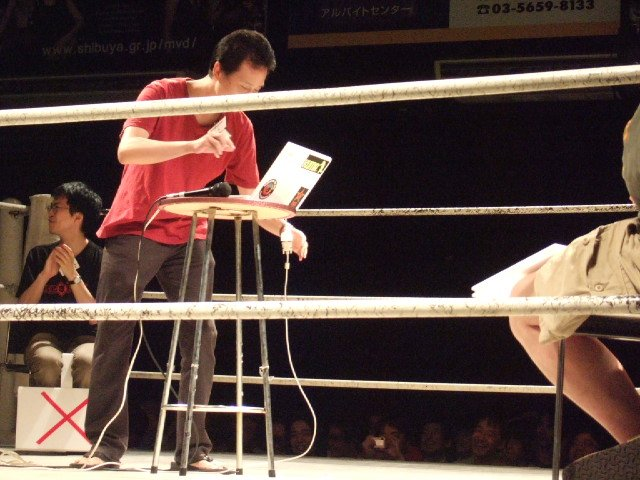
\includegraphics[width=1\hsize]{image200609/20060827-llgong.jpg}

%% さわださんここから
\dancersection{あなたが知らないうちに使っているDebian specific}{澤田さん}
\label{sec:sawadadebianspecific}

\subsection{はじめに}

Debianパッケージを管理するためのツールであるaptやdpkgなどは一目で
Debian specificとわかります。
しかし、日常的に利用しているコマンド、設定ファイルなど
でも実はDebian固有のものであったり
パッケージ化する際に変更が加えられていたりするものがあります。
ここではそのようなあなたの知らないDebian specificを紹介します。

\subsection{adduser}

Debianで

\begin{commandline}
# adduser hoge
\end{commandline}

を実行するとhogeユーザが作られパスワードの入力が求められます。
Fedoraで同じコマンドラインを実行した場合、hogeユーザは作られますが
パスワード入力は求められません。パスワードは別途passwdコマンドで設定する
必要があります。

この違いはDebianのadduserとFedoraでadduserの実体の違いによるものです。
Fedoraのadduserはuseraddへのシンボリックリンクです。
DebianのadduserはPerlスクリプトで、useradd、passwd等を
呼び出してユーザを作成しています\footnote{パスワード入力のプロンプトは
passwdコマンドが表示しています}。

ちなみに、FreeBSDのadduserはシェルスクリプトで書かれており、pwというコマ
ンドを呼び出すことでユーザの追加を行っているようです。
Debian GNU/kFreeBSDはFreeBSDカーネルの上にGNUのツールやglibc、Debianのツー
ルを乗せたものであるため、Debianのadduserが使われており、useraddとpasswd
でユーザの追加を行っていました。

\subsection{ifup}

ネットワークの設定を変えたのでインターフェースを再起動したいという場合、
Debianでは以下のコマンドラインを実行するとautoに設定されている
インターフェースをすべて再起動することができます。

\begin{commandline}
# ifdown -a \&\& ifup -a
\end{commandline}

一方Fedoraでは-aオプションは使えず、また、複数のインターフェースを指定す
ることはできません。

インターフェースの設定ファイルもDebianでは/etc/network/iterfaces、
Fedoraでは/etc/sysconfig/network-scripts/ifcfg-$<$インターフェース名$>$
となっており、フォーマットはまったく違います。

\subsection{Xsession}

startxのmanを見るとXの起動時に実行されるスクリプトは~/.xinitrcとなって
います。しかし、Debianでは~/.xsessionに書いておけばstartxを実行したと
きでもグラフィカルログインしたときでも同じ環境にすることができます。

これは、Debianでは素のXに対して変更を加えているためです。

startxしたときのフローは次のようになっています。
\begin{enumerate}
\item /usr/bin/startx
\item ~/.xinitrcがあったら~/.xinitrcを実行。なかったら
	  /etc/X11/xinit/xinitrc(Debian向けに修正されています)を実行
\item /etc/X11/Xsessionを実行
\end{enumerate}

グラフィカルログイン(xdm)した場合のフローは次のようになります。
\begin{enumerate}
\item /etc/X11/xdm/xdm-configのDisplayManager*sessionに書かれたコマンド
	  (通常、/etc/X11/xdm/Xsession(Debian向けに修正されています))を実行
\item /etc/X11/Xsessionを実行
\end{enumerate}

というわけでどちらの場合も/etc/X11/Xsessionが実行されます。
この/etc/X11/XsessionはDebian specificなもので/etc/X11/Xsession.dディレ
クトリにあるスクリプトを順に実行します。
このうち、50x11-common\_determine-startupで起動プログラムの検出が行われ、
~/.xsessionがある場合、~/.xsessionが起動プログラムに選ばれます。
99x11-common\_startで50x11-common\_determine-startupで選ばれたプログラム
が実行されることで~/.xsessionに書かれた内容が有効になります。

ちなみに、Fedoraでは~/.Xclientsに書くとstartxでもグラフィカルログインで
もスクリプトを実行してくれるようです。ただし、/etc/X11/Xsession.dディレ
クトリのような仕組みはないようです。

\subsection{lesspipe}

lessでgzip圧縮されたファイルを開こうとすると通常次のようになります。

\begin{commandline}
$ less hoge.txt.gz
"hoge.txt.gz" may be a binary file.  See it anyway?
\end{commandline}

ひょっとしたら上のようなメッセージは表示されずに
hoge.txtの内容が表示されている方もいらっしゃるかもしれません。
その場合、次の環境変数が設定されているはずです。

\begin{commandline}
$ printenv | grep ^LESS
LESS=-M
LESSOPEN=| /usr/bin/lesspipe '%s'
LESSCLOSE=/usr/bin/lesspipe '%s' '%s'
\end{commandline}

lessにはLESSOPENという環境変数が設定されているとファイルを読み込む前
にLESSOPENで指定されたコマンドにファイル名を渡してコマンドの標準出力をファ
イルの内容として読み込むという機能があります。
これにより、gzip圧縮されたファイルを

\begin{commandline}
$ less hoge.txt.gz
\end{commandline}

というコマンドラインで表示することができます。
また、この機能を応用することで

\begin{commandline}
$ less hoge.tar.gz
\end{commandline}

とした場合にtarされているファイルの一覧を取得するといったこともできます。

/usr/bin/lesspipeはDebian specificなものです。他のディストリビューション
にも同様の機能を持つものが含まれていることが多いのですが、Debianの
lesspipeは対応している拡張子の数が多いことが特徴です。

language-envを実行するとLESSOPENの設定をしてくれるため
気づかず使っているという方もいらっしゃるのではないでしょうか。

\subsection{Debian specificの見つけ方}

それがDebian specificであるか知るためにはmanを参照するという方法がありま
す。manを見ると、

\begin{commandline}
Debian GNU/Linux        Version 3.97        ADDUSER(8)
\end{commandline}

のように書かれているのでDebian specificと推測することができます。
しかし、それ以外にDebian specificかを知るよい方法はないようです。

Xsessionやlesspipeのようにオリジナルの配布内容からファイルが追加されてい
る場合、ソースパッケージのdebianディレクトリに追加ファイルが格納されてい
ます。
debianディレクトリにあるファイルリストからcontrolやpostinstなどの制御ファ
イルを除いたものを取得すればそのパッケージにDebian specificな変更があり
そうか推測することができると考えられます。

%% さわださんここまで
%% 小林さんここから
\dancersection{翻訳へのさそい}{小林儀匡}
\label{sec:honnyaku}

\subsection{はじめに}

国際化はDebianの一つの特徴です。
その国際化の達成には、
フレームワークの整備から各ソフトウェアの対応、
そしてメッセージやドキュメントの翻訳まで、
多岐に渡る非常に膨大な作業を必要とします。
ここでは、それらの作業のうち、
最も大量の作業を必要とする一方で一般ユーザが最も取り組みやすい翻訳に
ついて、
主にDebian JPまわりで行われている日本語訳作業をまとめます。

\subsection{共通の作業用インフラストラクチャ}

まず、
翻訳作業で共通に使われるインフラストラクチャをまとめて説明します。
これらは、後述する各種作業の説明でも頻繁に登場します。

\subsubsection{作業用メーリングリスト}

翻訳作業に関するやりとりには主にメーリングリストが使われます。
Debian本家のものとDebian JPのものがありますが、どちらについても、
翻訳関連のメーリングリストは誰でも (DebianおよびDebian JPのメンバーで
なくても) 自由に参加できます。

日本語訳関連の作業に関するやりとりによく使われるのは、
Debian JPのdebian-doc\footnote{\texttt{debian-doc@debian.or.jp}}および
debian-www\footnote{\texttt{debian-www@debian.or.jp}}メーリングリストです。
登録に使うアドレスは、
それぞれ\texttt{debian-doc-ctl@debian.or.jp}と
\texttt{debian-www-ctl@debian.or.jp}です。
これらのメーリングリストに関する情報が、
\url{http://www.debian.or.jp/MailingList.html}\footnote{%
準備中の新サイトでは
\url{http://www-internal.debian.or.jp/community/ml/}。}にあるので、
参照してください。
過去にこれらのメーリングリストに投稿されたメールのアーカイブは、
\url{http://lists.debian.or.jp/debian-doc/}および
\url{http://lists.debian.or.jp/debian-www/}で完全に公開されています。

さらに、パッケージの更新に伴うdebconf-poの翻訳更新の依頼など、
Debian本家の開発者との英語でのやりとりには、
主にDebian本家のdebian-japaneseメーリングリスト\footnote{%
\texttt{debian-japanese@lists.debian.org}}が使われます。
登録およびアーカイブは\url{http://lists.debian.org/debian-japanese/}で
利用可能です。
メーリングリストを経由せずに、前のバージョンの翻訳者や、
翻訳者として活発に活動されているかた、
あるいは本家で活動している日本人開発者のところに直接メールが行ったりする
こともあります。

また、
ドキュメントの翻訳ならDebian本家のdebian-docメーリングリスト\footnote{%
\texttt{debian-doc@lists.debian.org}}に、
ウェブページの翻訳ならDebian本家のdebian-wwwメーリングリスト\footnote{%
\texttt{debian-www@lists.debian.org}}にそれぞれ登録しておくと、
内容に関する質問や間違いの修正などに関するやりとりを本家の方々とできます。
それぞれ\url{http://lists.debian.org/debian-doc/}および
\url{http://lists.debian.org/debian-www/}で、
登録やアーカイブ閲覧ができます。

\subsubsection{対訳表}

日本語訳の対訳表は、Debian JP debian-docメーリングリストでたまに
話題になりますが、なかなか整備までいかないのが現状です。
メーリングリストで訳語に関する問い合わせをしたり、
査読依頼を出してコメントをもらったりできるので、
そこまで気になることはないでしょう。
一応、既存のいくつかの対訳表をポインタとして示しておきます。
\begin{itemize}
 \item Debian JPの『略語の解説』:
       \url{http://www.debian.or.jp/devel/abbreviation.html}
 \item Debian JP対訳表
       \begin{itemize}
	\item ソース: \url{http://www.debian.or.jp/Documents/trans_table/}
	\item HTMLでの出力:
	      \url{http://www.debian.or.jp/Documents/trans_table/trans_table.html}
	\item dict形式での出力:
	      \url{http://www.debian.or.jp/Documents/trans_table/trans_table.dict}
       \end{itemize}
 \item APT, dpkg関連の表記に関する用語集 (武藤健志さんのWiki):
       \url{http://kmuto.jp/open.cgi?DebianGlossary}
 \item かねこさんによる『Security関連用語対訳集』:
       \url{http://lists.debian.or.jp/debian-www/200607/msg00120.html}
 \item 小林によるDebian Weekly News関連のja.po\footnote{Debian Weekly
       News用wmlファイルの後半のSecurity UpdatesおよびRemoved Packagesから
       用語を抽出してpoとしたものです。}:
       \url{http://dolphin.c.u-tokyo.ac.jp/~nori1/dwn/ja.po}
\end{itemize}

対訳表というわけではありませんが、
これらの他に小林が訳語の選択によく利用するのは、Googleです。
Debianのウェブサイト全般から訳語を探したければ「site:www.debian.org」を、
Debian Weekly Newsから探したければ「site:www.debian.org/News/weekly」を
つけて検索し、引っ掛かったページを見ながら訳語を決めるということをよく
やっています。

\subsection{各種ソフトウェアのpoや付属ドキュメントの翻訳}

\subsubsection{作業方法}

各種ソフトウェアのメッセージカタログ (po) や付属ドキュメント、
manpageなどの翻訳に関する議論は、
Debian JPのdebian-docメーリングリストで行われています。
これらの翻訳はソフトウェアの更新に伴って更新作業をする必要があるので、
主に開発元 (upstream) のソフトウェア作者などと (主に英語で) やりとりを
しながら作業することになります。
しかし、特にDebianと密接に関連したソフトウェアについては訳語が統一されて
いるほうがよいので、
訳語選択などについてdebian-docメーリングリストで査読を依頼することが
推奨されています。

\subsubsection{翻訳状況の確認}

poについては、翻訳状況に関する情報が以下のページで得られます。
\begin{itemize}
 \item poファイル翻訳のページ (%
       \url{http://www.debian.org/international/l10n/po/})
       \begin{itemize}
	\item 日本語の翻訳状況:
	      \url{http://www.debian.org/international/l10n/po/ja}
	\item 言語ごとの翻訳ランキング:
	      \url{http://www.debian.org/international/l10n/po/rank}
       \end{itemize}
 \item Debian-Installerの各言語翻訳状況
       \begin{itemize}
	\item 不安定版 (unstable):
	      \url{http://d-i.alioth.debian.org/l10n-stats/translation-status.html}
	\item テスト版 (testing):
	      \url{http://d-i.alioth.debian.org/l10n-stats/translation-status-testing.html}
       \end{itemize}
\end{itemize}

\subsection{debconf-po関連}

\subsubsection{debconf-poとは}

debconf-poとは、
Debianパッケージをインストールする際になされる設定関連の質問 (debconfの
質問) に翻訳を提供し、
localizeされたインタフェースでユーザが質問に答えられるようにするための
poファイルです。

例えば、sargeで\texttt{locales}パッケージを設定する場合、
英語のロケールでは次のような画面が現れます。\\
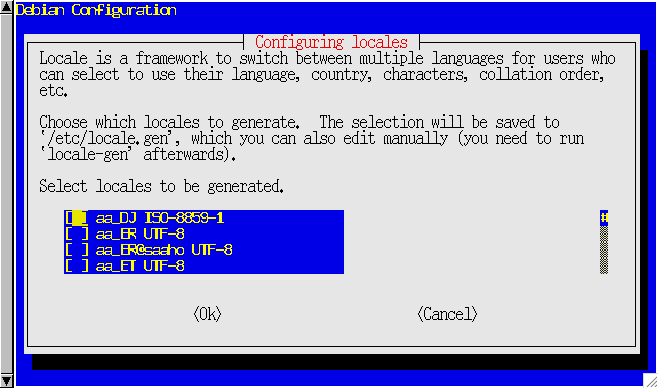
\includegraphics[width=1\hsize]{image200609/debconf-en.png}\\
これに対して日本語のロケールでは次のようになります。\\
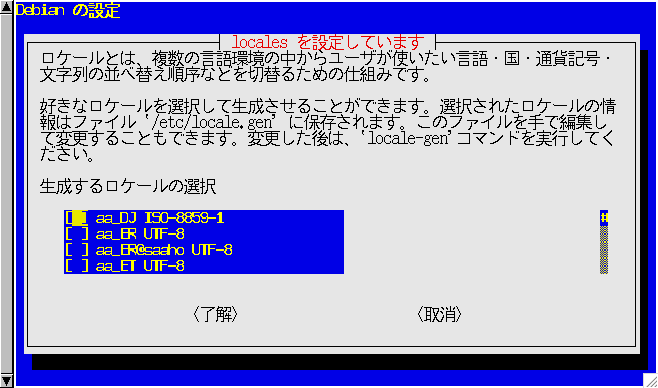
\includegraphics[width=1\hsize]{image200609/debconf-ja.png}\\
このようにロケールに応じた質問を提供するのがdebconf-poです。

このdebconfの質問自体は、次のように、パッケージ作者によって、
ソースパッケージのdebianディレクトリの下の
バイナリパッケージ用templatesファイルに英語で書かれています。\\
\begin{commandline}
Template: locales/locales_to_be_generated
Type: multiselect
Choices: ${locales}
_Description: Select locales to be generated.
 Locale is a framework to switch between multiple languages for users who can
 select to use their language, country, characters, collation order, etc.
 .
 Choose which locales to generate.  The selection will be saved to
 `/etc/locale.gen', which you can also edit manually (you need to run
 `locale-gen' afterwards).

Template: locales/default_environment_locale
Type: select
_Choices: None, ${locales}
Default: None
_Description: Which locale should be the default in the system environment?
 Many packages in Debian use locales to display text in the correct
 language for users. You can change the default locale if you're not
 a native English speaker.
 These choices are based on which locales you have chosen to generate.
 .
 Note: This will select the language for your whole system. If you're
 running a multi-user system where not all of your users speak the language
 of your choice, then they will run into difficulties and you might want
 not to set a default locale.

\end{commandline}

オリジナルは英語ですが、非英語圏のユーザにとっては、
自分の母語で質問されるほうがよいでしょう。
そこで、localizeされたdebconf質問をユーザが利用できるようにするのが、
このdebconf-poです。

\subsubsection{作業方法}

作業を開始する前に、
まずは\ref{subsubsec:debconf-po-check}で述べる翻訳状況調整ページで
既に翻訳作業が行われていないか確認するとよいでしょう。
その上で翻訳対象とするパッケージを決めたら、
\url{http://www.debian.org/intl/l10n/po-debconf/pot}からそのファイルの
templates.potファイルをダウンロードします。
もちろん、ソースパッケージを手に入れ、
目的のバイナリパッケージのtemplatesファイルに対して
\texttt{po-debconf}パッケージの\texttt{debconf-gettextize}コマンドを
実行し、templates.potを生成してもかまいません。

templates.potファイルを取得したら、
名前をja.poに変更した上で翻訳しましょう。

翻訳を終えたら該当パッケージにseverityを「wishlist」、tagsを「l10n,
patch」としてバグ報告しましょう。
ただ、慣れていないうちはDebian JPのdebian-docメーリングリストで
査読してもらうことを強くお勧めします。

% FIXME: 余裕があったらもっと書く!!

\subsubsection{翻訳状況の確認}
\label{subsubsec:debconf-po-check}

debconf-poについては、翻訳状況に関する情報が以下のページで得られます。
\begin{itemize}
 \item debconf-poファイル翻訳のページ (%
       \url{http://www.debian.org/international/l10n/po-debconf/})
       \begin{itemize}
	\item 日本語の翻訳状況:
	      \url{http://www.debian.org/international/l10n/po-debconf/ja}
	\item 言語ごとの翻訳ランキング:
	      \url{http://www.debian.org/international/l10n/po-debconf/rank}
       \end{itemize}
 \item 武藤健志さんが提供するdebconf-po日本語翻訳作業調整ページ (%
	    \url{http://kmuto.jp/debian/po-trans/})
       各パッケージのdebconf-poの翻訳状況および最終訳者の情報を
       得ることができます。
\end{itemize}

\subsection{ウェブページ関連}

\subsubsection{Debianウェブページの仕組み}

DebianのウェブページはWMLというファイル形式を利用しています。
WMLとはウェブサイトメタ言語 (web site meta language) のことで、
Debianでは\texttt{wml}パッケージとして提供されています。
ここでは詳しくは述べませんが、
翻訳が原文に追従できているかの確認などがこのWMLの機構を用いて
行われている、ということだけ書いておきます。

次の例は、
\url{http://www.debian.org/News/weekly/2006/35/index}のソースとなってい
る、\texttt{cvs.debian.org}の\texttt{webwml}モジュール\footnote{%
\url{http://cvs.debian.org/?root=webwml}}の、
\texttt{webwml/japanese/News/weekly/2006/35/index.wml}です。\\
\begin{commandline}
#use wml::debian::weeklynews::header PUBDATE="2006-08-29"
 #SUMMARY="Firmware, FrOSCon, Events, Cuba, Translations, GIT, Sarge,
 #Etch" 
#use wml::debian::translation-check translation="1.8"

<p>Welcome to this year's 35th issue of DWN, the weekly newsletter for the
Debian community.  Bug squashing parties have been announced for September 8th
to 10th in <a
href="http://lists.debian.org/debian-devel-announce/2006/08/msg00012.html">\
Vienna</a> and for September 15th to 17th in <a
href="http://lists.debian.org/debian-devel-announce/2006/08/msg00013.html">\
J&uuml;lich</a>, Germany.  OSDir has taken <a
href="http://shots.osdir.com/slideshows/slideshow.php?release=724&amp;slide=2">\
Debian installer</a>.  Petr Stehlik <a
href="http://lists.debian.org/debian-68k/2006/08/msg00234.html">reported</a>
that the installation of <a href="$(HOME)/releases/sarge/">sarge</a> and <a
href="$(HOME)/releases/etch/">etch</a> worked flawlessly in the recently <a
href="http://lists.debian.org/debian-68k/2006/08/msg00226.html">fixed</a>
version of <a href="http://packages.debian.org/aranym">ARAnyM</a>, a 32bit
Atari ST/TT/Falcon virtual machine.</p>

[snip]

#use wml::debian::weeklynews::footer editor="Sebastian Feltel, Mohammed
 Adn&egrave;ne Trojette, Tobias Toedter, Martin 'Joey' Schulze" 
\end{commandline}

このうち\verb|#|で始まる行がWMLの命令です。
例えば、\\
\begin{commandline}
#use wml::debian::translation-check translation="1.8"
\end{commandline}

という行は、原文 (\texttt{webwml/english/News/weekly/2006/35/index.wml})
のr1.8に基づいているという意味です。

\subsubsection{作業方法}

翻訳作業を開始するには、目的のページのWMLファイルを入手する必要があります。
CVSを使い慣れている場合は、
コマンドラインから日本語のツリー (\texttt{webwml/japanese}) と
英語のツリー (\texttt{webwml/english}) をチェックアウトすると
よいでしょう。
CVSを使い慣れていない場合は\url{http://cvs.debian.org/?root=webwml}から
リポジトリビューアViewCVSを使って英語または日本語の目的のファイルを
ダウンロードしましょう。
ただし、この方法では後述するlatin-1文字の置換作業ができないため、
ページ内にlatin-1文字が含まれていた場合には自分で何とかして
対処しなければなりません。
したがって、こちらはあまりお勧めしません。

新規翻訳の場合、英語のファイルを取得したら、
まずはそれを日本語訳用に変換しなければなりません。
それには\texttt{webwml/copypage.pl}を用いて次のように実行します。\\
\begin{commandline}
nori1[6:12]%  DWWW_LANG=japanese ./copypage.pl english/News/weekly/2006/37/index.wml
Unable to open language.conf. Using environment variables...
Processing english/News/weekly/2006/37/index.wml...
Destination directory japanese/News/weekly/2006/37/ does not exist,
Copied News/weekly/2006/37/index.wml, remember to edit japanese/News/weekly/2006/37/index.wml
\end{commandline}

こうすると、オリジナルのファイルのリビジョンを元にして、
前述の\texttt{wml::debian::translation-check translation}の値が適切に
設定されます。
また、latin-1でエンコードされた文字列があっても適切な文字実体参照に
置換され、
日本語の文字と欧米の文字が共存できるようになります。
あとは自由に翻訳してください。

新規翻訳ではなく、翻訳が古くなったページの更新であれば、
英語のページを日本語用にコピーする必要はありません。
\texttt{wml::debian::translation-check translation}の値を適切に設定し、
原文の差分を見ながら翻訳を更新しましょう。

翻訳の際のルールについては、
\url{http://www.debian.or.jp/devel/www/WebTranslation.html}を参照すると
よいでしょう。
また、
ウェブページはMozilla FirefoxのようなGUIのウェブブラウザでもw3mのような
テキストブラウザでも美しく見えてほしいので、
改行位置には気をつけることになっています。
\url{http://lists.debian.or.jp/debian-www/200408/msg00046.html}や
\url{http://lists.debian.or.jp/debian-www/200609/msg00102.html}などを
参考にしてください。

翻訳が終わったら、
Debian JPのdebian-wwwメーリングリストに査読・コミット依頼を出します。
現在はコミットは主に今井伸広さんがしてくださっています。

% FIXME: 余裕があったらもっと書く!!

\subsubsection{翻訳状況の確認}
\label{subsubsec:www-check}

ウェブページについては、翻訳状況に関する情報が以下のページで得られます。
\begin{description}
 \item[ウェブサイト翻訳状況
	    (\url{http://www.debian.org/devel/website/stats/})] 
	    言語ごとの翻訳状況の統計が載っています。
 \item[日本語のウェブサイト翻訳状況
	    (\url{http://www.debian.org/devel/website/stats/ja.html})] 
	    日本語の各ファイルの翻訳状況がわかります。
\end{description}

\subsection{The Debian Description Translation Project (DDTP)}

\subsubsection{DDTPとは}

Debian Description Translation Project (DDTP) とは、
現在すべて英語で提供されているDebianパッケージ説明文 (Description) に
翻訳を提供し、
それらの翻訳情報が使えるインフラを整えようというプロジェクトです。
\url{http://ddtp.debian.net/}がプロジェクトのウェブサイトです。

おそらく皆さん御存知でしょうが、
パッケージ説明文とはパッケージ付随情報の一つで、
パッケージの内容を説明するとともに、
\texttt{aptitude search}などでパッケージを検索する際に便利になるよう
提供されています。
以下は、sargeで\texttt{aptitude}パッケージの情報を表示させたときの
様子で、「詳細:」で始まる行\footnote{aptitude
0.4.2以降では「説明文:」という訳語に変わっています。}以降が
パッケージ説明文です。\\
\begin{commandline}
nori1[12:04]%  aptitude show aptitude            whale:~/svnwc/deb/skkdic/trunk
パッケージ: aptitude
ステータス: インストール済み
自動的にインストールされる: no
バージョン: 0.2.15.9-6bpo3
優先度: 任意
分類: admin
保守担当者: Daniel Burrows <dburrows@debian.org>
展開サイズ: 5288k
依存: libapt-pkg-libc6.3-5-3.11, libc6 (>= 2.3.2.ds1-21), libgcc1 (>=
      1:3.4.1-3), libncurses5 (>= 5.4-1), libsigc++-1.2-5c102, libstdc++5 (>=
      1:3.3.4-1)
提案: aptitude-doc-en | aptitude-doc
詳細: terminal-based apt frontend
 aptitude is a terminal-based apt frontend with a number of useful features,
 including: a mutt-like syntax for matching packages in a flexible manner,
 dselect-like persistence of user actions, the ability to retrieve and display
 the Debian changelog of most packages, and extreme flexibility and
 customization.

 aptitude is also Y2K-compliant, non-fattening, naturally cleansing, and
 housebroken.

\end{commandline}

このパッケージ説明文のエントリ自体は、次のように、パッケージ作者によって、
ソースパッケージのdebian/controlファイルに英語で書かれています。\\
\begin{commandline}
[snip]
Description: terminal-based apt frontend
 aptitude is a terminal-based apt frontend with a number of useful
 features, including: a mutt-like syntax for matching packages in a
 flexible manner, dselect-like persistence of user actions, the
 ability to retrieve and display the Debian changelog of most
 packages, and extreme flexibility and customization.
 .
 aptitude is also Y2K-compliant, non-fattening, naturally cleansing,
 and housebroken.
[snip]
\end{commandline}

説明文は、\verb|Description:|と同じ行に書かれるshort descriptionと、
その後のlong descriptionに分かれます。

オリジナルは英語ですが、非英語圏のユーザにとっては、
自分の母語でパッケージ説明文を読めるほうがよいでしょう。
そこで、localizeされたパッケージ説明文をユーザが利用できるようにする
ことを目的として作られたのがこのDDTPというプロジェクトです。

このプロジェクトは数年前から存在しており、
日本語についても日本語チームコーディネータの田村一平さんなどが
積極的に作業を進め、
一時は翻訳率でトップになったこともありました\footnote{%
\url{http://d.hatena.ne.jp/denson/20050315/p2}}が、
Debianのホストの問題で暫く停止していました。
完全にではありませんが、
最近ようやく復活の兆しが見え始めました\footnote{%
\url{http://www.debian.org/News/weekly/2006/31/}や
\url{http://www.debian.org/News/weekly/2006/35/}に関連記事があります。
\url{http://lists.debian.org/debian-devel/2006/07/msg01323.html}から
始まる ``Translated packages descriptions progress'' というスレッドも
盛り上がっていました。}。
最近は以下のような状況です。
\begin{itemize}
 \item Debian本家のウェブサイトにもDDTPのページ
       \footnote{\url{http://www.debian.org/international/l10n/ddtp}}が
       作られた。
 \item プロジェクトウェブサイトが復活し、翻訳状況を見られるようになった。
 \item メールインタフェース (後述) が復活した。
 \item ウェブインタフェース (後述) が作られた。
\end{itemize}

\subsubsection{作業方法}

DDTPの作業方法については、
Debian JPのサイトに日本語の説明があります\footnote{%
\url{http://www.debian.or.jp/devel/doc/Description-ja.html}}。
ただしこれは復活前のもので情報がやや古くなっているので、
最近作られたDebian本家のウェブサイトのDDTPのページ\footnote{%
\url{http://www.debian.org/international/l10n/ddtp}}を参照するのが
よいでしょう。
このページは本資料執筆現在は英語でしか利用できないので、
ここでは本家の説明に基づいて、簡単に説明します\footnote{%
本家のDDTPのページは近々日本語で利用可能になる予定です。
今後はDebian JPのページではなくそちらのページをメインの日本語情報として
参照するとよいでしょう。}。

\subsubsubsection{メールインタフェース}

DDTPは、誰でも気軽に作業できるよう、
非常に簡単なインタフェースを通じて作業できるようになっています。
現在Debianパッケージ数は15000を超えており、
debconfとは異なりパッケージ説明文はすべてのパッケージに含まれているので、
それらをすべてlocalizeしようという目的をもつこのプロジェクトは、
とても壮大で大量のマンパワーを必要とするからです。
新しいパッケージでパッケージ説明文が改良されることがあるので、
それらの変化にも追従できなければいけません。

公式インタフェースはメールで、
それ以外にもウェブインタフェースが開発されています。

メールインタフェースを使うには、
次のような件名 (Subject) で\texttt{pdesc@ddtp.debian.net}にメールを
送ってください。\\
\begin{commandline}
GET n lang
\end{commandline}

\texttt{n}はパッケージ説明文の数で、9以下の数値を指定してください。
\texttt{lang}は言語コードで、日本語では\texttt{ja}です。
\texttt{lang}の後ろにドット (\texttt{.}) に繋げてエンコーディングを
指定することも可能です。

メールを送ると、
指定された数だけパッケージ説明文が添付されたメールが返信されます。
これらのパッケージ説明文はしばらくの時間ロックされ、
メールで取り寄せた人のみが作業できるようになるので、
安心してゆっくり作業しましょう。
各添付ファイルは次のような形式になっているので、
パッケージ説明文中の\texttt{<trans>}と記された部分を翻訳してください。\\
\begin{commandline}

# Source: aolserver4-nsopenssl
# Package(s): aolserver4-nsopenssl
# Prioritize: 45
# This Description is active
# This Description is owned
Description: AOLserver 4 module: module for SSL mode.
 This module adds SSL capabilities to aolserver, and gives Tcl scripts
 an API to access openssl functions.
 .
 This is currently a beta release! Use at your own risk.
Description-ja.euc-jp: <trans>
 <trans>
 .
 <trans>
#
# other Descriptions of the aolserver4-nsopenssl package with a translation in ja:
# 
\end{commandline}

翻訳するのは、\texttt{<trans>}だけです。
英語のパッケージ説明文は変更しないでください\footnote{誤りを発見したら
そのパッケージのバグとしてBTSにバグ報告してください。}。
また、ドットだけの行も段落のセパレータとして重要なので、
変更を加えないでください。
ただし、
上の例ではshort descriptionとlong descriptionの各段落の内容がすべて
\texttt{<trans>}となっていますが、
一部の段落に既に翻訳が入っている場合もあります。
それは、他のパッケージに同じ段落が含まれておりそれが翻訳済みの場合です。
これらは修正してもかまいません。

エンコーディングは正しいものを用いるよう注意してください。
例えば、
\texttt{GET 1 ja}という件名でパッケージ説明文を取り寄せると、
\texttt{GET 1 ja.euc-jp noguide}という件名のメールが返ってきます。
これは、日本語のデフォルトエンコーディングがEUC-JPとなっているからです。
この場合、翻訳したファイルのエンコーディングはEUC-JPとし、
メールで送る際にもISO-2022-JPで送ってしまわないよう気をつけてください。
ただし、上の例の翻訳部のフィールドが\texttt{Description-ja.euc-jp}と
なっていることからもわかるように、
エンコーディング指定は変更可能です。
UTF-8がいいというのであれば、
フィールド名を\texttt{Description-ja.UTF-8}として翻訳文字列をUTF-8で
記入してください。

翻訳を終えたらファイルを\texttt{pdesc@ddtp.debian.net}に送り返します。
翻訳文はbase64エンコードするとよいでしょう。
中野武雄さん作のddts-send\footnote{%
\url{http://surf.ap.seikei.ac.jp/~nakano/linux/ddts-send.ja.html}}や
\texttt{ddtc}パッケージ\footnote{%
\url{http://packages.debian.org/ddtc}}などのヘルパーも利用可能です。

\subsubsubsection{ウェブインタフェース}

Martijn van Oosterhoutさんが作成したウェブインタフェースはDDTSSと呼ばれ、
\url{http://kleptog.org/cgi-bin/ddtss2-cgi/xx}にあります。
翻訳と査読・校正の作業をウェブで簡単に行えるようになっています。

% FIXME: もっと書く!!

\subsubsection{翻訳状況の確認}

DDTPでは、翻訳状況の確認は以下のページでできます。

\begin{description}
 \item[プロジェクトウェブサイト (\url{http://ddtp.debian.net/})]
	    トップページには言語ごとの翻訳状況の統計が載っています。
	    パッケージごとに各言語への翻訳状況を表示することも可能です。
\end{description}

\subsubsection{翻訳内容の取得}

DDTPによるパッケージ説明文の翻訳は、Debianのミラーの
\url{http://ftp.jp.debian.org/debian/dists/sid/main/i18n/}などから
取得可能です。
例えば日本語なら、上記のディレクトリのTranslation-ja.gzや
Translation-ja.bz2が利用できます。

\subsection{おわりに}

本節では、国際化の一環として重要な翻訳について、
作業方法および各種情報を取得できるページをざっと説明しました。
翻訳は非常に手間がかかる作業で、膨大なマンパワーを必要とします。
Debianではあなたの参加を心待ちにしています。

\subsection{参考文献}

以下のページも参考にしてください。

\begin{itemize}
 \item 武藤健志さんのblogの『Debianドキュメント翻訳手続き』:
       \url{http://kmuto.jp/d/index.cgi/debian/debian-doc-procedure.htm}
\end{itemize}

%% 小林さんここまで

\dancersection{dpkg, apt のプロファイリング}{上川}
\label{sec:dancerjapt}

apt や dpkg のどの部分が一番遅いのか、実際にプロファイリングしてみます。
この例をケーススタディーとして一般的にどういう作業をすればパフォーマンス
チューニングが必要な部分を抽出できるのか、をあきらかにしてみましょう。

\subsection{oprofile のインストールと設定方法}

Debianのデフォルトのカーネルはoprofileをサポートしています
\footnote{i386, amd64 などのアーキテクチャ以外での利用は現時点では難し
い可能性があるので確認してください。} 。もし、自分でコンパイルしていたり
して oprofile サポートを追加していない場合は、カーネルを oprofile サポー
ト付きでコンパイルしなおします。オプションは \texttt{CONFIG\_OPROFILE}
です。メニューでは

\texttt{Intrumentation support : Profiling Support :
Oprofile system profiling (experimental)}\footnote{2.6.18-rc1 現在}

にあります。

カーネルがサポートしている場合、oprofileを利用するのに追加で必要なのは
\texttt{oprofile}パッケージです。
\texttt{apt-get install oprofile}でインストールしましょう。

カーネルのシンボルのプロファイリング\footnote{無い場合はカーネルの内部の
どこかで実行していることはわかるが、実際どの関数で時間がかかっているのか、
ということがわからない}をするために、vmlinuxファイルが必要です。
カーネルを自分でコンパイルした場合には、ビルドしたディレクトリに
vmlinux ファイルがあります。 make-kpkg を利用してビルドしたのであれば、

\begin{commandline}
 /lib/modules/$(uname -r)/build
\end{commandline}

から適切にリンクがはられているはずです。探してみてください。
\footnote{oprofile メーリングリストには vmlinux ファイルよりは普及している System.map を利用するパッチ
というのも存在するので、それを適用してみるのもよいかもしれません。}

\subsection{oprofile が自分の利用しているCPUをサポートしていない場合}

残念ながら9月現在時点の Debian Package では、Intel core duo CPU 上では 
oprofile が動作しません。oprofile は認識できていない場合、cpu\_type 変数
が unset という値になります。カーネル側は cpu\_type として i386/core を
出力しているので、この時点でどうやらカーネル側のサポートは追加されている
らしいということがわかります。

\begin{commandline}
$ sudo opcontrol --init
cpu_type 'unset' is not valid
$ opcontrol --list-events
Unable to open cpu_type file for reading
Make sure you have done opcontrol --init
cpu_type 'unset' is not valid
$ cat /dev/oprofile/cpu_type
i386/core
$ uname -a
Linux coreduo 2.6.18-rc1dancer #2 SMP Sun Jul 9 09:57:01 JST 2006 i686 GNU/Linux
\end{commandline}

プロファイルを取得するという目的を考えると手段としてはいくつか考えられます。

\begin{itemize}
 \item プロファイルの仕組はあまりかわらないだろうと見込み、
       \url{arch/i386/oprofile/nmi_int.c}の ppro\_init を修正、
       piiiとかに見せてしまう

 \item まじめにoprofileのユーザ空間アプリケーションを修正、core duo の
       仕様書を読み、対応を追加

 \item おそらくすでに修正されていることを見越して、oprofile の CVS レポ
       ジトリをみにいく       

 \item 実験することが目的なのでサポートされているCPUのマシンを準備する

\end{itemize}

今回はoprofileの開発メーリングリストを見たところ、5月の時点でだれかがパッ
チを書いているのを発見したので、それをとりこみます。
念のため、今後作業する人のためにBTSにも登録しました。\debianbug{380462}

確認してみると、どうやら動作してくれていることがわかりました。ここで、当
面重要なのは、 CPU\_CLK\_UNHALTED でしょう。CPUサイクルがどの関数で消費
されているのかということをトラッキングできます。まずCPUの処理負荷がかかっ
ている部分を目視して、何か問題がないかを眺めてみて、何も問題なく、それな
りに問題が追求できにくくなった後に、L2キャッシュのイベントの発生度合とか
を確認していけばよいでしょう。

\begin{commandline}
$ sudo opcontrol --init
$ sudo opcontrol --list-events
oprofile: available events for CPU type "Core Solo / Duo"

See Intel Architecture Developer's Manual Volume 3, Appendix A and
Intel Architecture Optimization Reference Manual (730795-001)

CPU_CLK_UNHALTED: (counter: all)
        Unhalted clock cycles (min count: 6000)
        Unit masks (default 0x0)
        ----------
        0x00: Unhalted core cycles
        0x01: Unhalted bus cycles
        0x02: Unhalted bus cycles of this core while the other core is halted
INST_RETIRED: (counter: all)
        number of instructions retired (min count: 6000)
L2_RQSTS: (counter: all)
        number of L2 requests (min count: 6000)
        Unit masks (default 0xf)
        ----------
        0x08: (M)odified cache state
        0x04: (E)xclusive cache state
        0x02: (S)hared cache state
        0x01: (I)nvalid cache state
        0x0f: All cache states
        0x10: HW prefetched line only
        0x20: all prefetched line w/o regarding mask 0x10.

[省略]

\end{commandline}

\subsection{デバッグシンボルを収集する:dpkg と apt をコンパイルしなおす}

まず、デバッグ情報がすでにあるパッケージについては、インストールします。
今回では、大きいものとして、libc6-dbg パッケージがあるので、それはインス
トールします。プロファイルの結果、イメージが上位に出現するなどで、必要そ
うであれば、あとで他のライブラリなどについてもデバッグ情報のあるバージョ
ンを追加しましょう。

今回プロファイル対象の dpkg と apt はデフォルトではデバッグ情報がありませ
ん、プロファイル出力を確認しやすいように、デバッグシンボルを追加してコン
パイルしなおします。

\begin{commandline}
 $ debuild -e DEB_BUILD_OPTIONS=nostrip
\end{commandline}
%$

その後、インストールします。

まず、oprofileを実行するのを便利にするために、スクリプトを仕込みます。
入力されたコマンドを10回実行してそのプロファイルを取得するというものです。

\begin{commandline}
 read CMD
 sudo opcontrol --shutdown
 sudo opcontrol --reset
 sudo opcontrol --setup \
  --vmlinux=/lib/modules/$(uname -r)/build/vmlinux \
    --event=CPU_CLK_UNHALTED:180000:0:1:1 --separate=library
    sudo opcontrol --start
 for A in $(seq 1 10); do
   $CMD
 done
 opcontrol --dump && \
 opreport -l -p /lib/modules/$(uname -r)/kernel 2>/dev/null \
  | head -30
\end{commandline}

まず、デバッグ用のバイナリが正常に作成できているか簡単に確認します。まず、
apt-get update をループでまわしてみます。libapt-pkgのシンボルレベルで確
認できているので、デバッグシンボルが存在しているということがわかります。

\begin{commandline}
sudo apt-get update
[中略]
CPU: Core Solo / Duo, speed 1833 MHz (estimated)
Counted CPU_CLK_UNHALTED events (Unhalted clock cycles) with a unit mask of 0x00 (Unhalted core cycles) count 180000
samples  %        image name               app name                 symbol name
23823    46.3519  libapt-pkg-libc6.3-6.so.3.11.0 apt-get                  
SHA1Transform(unsigned int*, unsigned char const*)
12732    24.7724  libapt-pkg-libc6.3-6.so.3.11.0 apt-get
 MD5Transform(unsigned int*, unsigned int const*) 
4282      8.3314  processor.ko             processor                acpi_processor_idle
2584      5.0276  libc-2.3.6.so            apt-get                  (no symbols)
2012      3.9147  vmlinux                  vmlinux                  __copy_to_user_ll
503       0.9787  gpgv                     gpgv                     (no symbols)
222       0.4319  vmlinux                  vmlinux                  timer_interrupt
166       0.3230  libapt-pkg-libc6.3-6.so.3.11.0 apt-get
 MD5Summation::Add(unsigned char const*, unsigned long) 
160       0.3113  vmlinux                  vmlinux                  page_fault
158       0.3074  libapt-pkg-libc6.3-6.so.3.11.0 apt-get
 SHA1Summation::Add(unsigned char const*, unsigned long) 
140       0.2724  libstdc++.so.6.0.8       apt-get                  (no symbols)
134       0.2607  vmlinux                  vmlinux                  find_get_page
125       0.2432  ld-2.3.6.so              http                     do_lookup_x
123       0.2393  vmlinux                  vmlinux                  sysenter_past_esp
95        0.1848  libapt-pkg-libc6.3-6.so.3.11.0 apt-get                  .plt
94        0.1829  ld-2.3.6.so              gpgv                     do_lookup_x
89        0.1732  libc-2.3.6.so            http                     (no symbols)
89        0.1732  vmlinux                  vmlinux                  do_generic_mapping_read
88        0.1712  ld-2.3.6.so              file                     do_lookup_x
87        0.1693  vmlinux                  vmlinux                  memcpy
72        0.1401  ld-2.3.6.so              http                     strcmp
69        0.1343  vmlinux                  vmlinux                  _spin_lock
65        0.1265  vmlinux                  vmlinux                  vfs_read
64        0.1245  ld-2.3.6.so              gpgv                     _dl_elf_hash
62        0.1206  vmlinux                  vmlinux                  __handle_mm_fault
60        0.1167  ld-2.3.6.so              http                     _dl_elf_hash
58        0.1128  oprofiled                oprofiled                (no symbols)
\end{commandline}

dpkgについてもプロファイリングしてみます。\footnote{ここで問題が出ました。
libc6 の dbg パッケージの情報を oprofile が処理できていないようです。
straceで解析してみましたが、ファイルをひらくところまでは何かできているよ
うです。これは別途バグ報告してみます。\debianbug{385704}}

\begin{commandline}
sudo dpkg -i ../dselect_1.13.22_i386.deb
[中略]
CPU: Core Solo / Duo, speed 1833 MHz (estimated)
Counted CPU_CLK_UNHALTED events (Unhalted clock cycles) with a unit mask of 0x00 (Unhalted core cycles) count 180000
samples  %        image name               app name                 symbol name
41009    32.6009  libc-2.3.6.so            dpkg                     (no symbols)
27485    21.8497  processor.ko             processor                acpi_processor_idle
14863    11.8156  dpkg                     dpkg                     parsedb
4845      3.8516  dpkg                     dpkg                     findnamenode
2691      2.1393  dpkg                     dpkg                     findpackage
1994      1.5852  dpkg                     dpkg                     f_dependency
1742      1.3848  vmlinux                  vmlinux                  get_page_from_freelist
1660      1.3196  dpkg-deb                 dpkg-deb                 inflate_fast
1552      1.2338  dpkg                     dpkg                     iterpkgnext
1520      1.2084  dpkg                     dpkg                     .plt
1500      1.1925  dpkg                     dpkg                     varbufaddbuf
1192      0.9476  dpkg                     dpkg                     filesdbinit
1080      0.8586  dpkg                     dpkg                     w_dependency
1001      0.7958  dpkg                     dpkg                     varbufdependency
988       0.7854  dpkg                     dpkg                     nfmalloc
884       0.7028  dpkg                     dpkg                     illegal_packagename
849       0.6749  vmlinux                  vmlinux                  page_fault
802       0.6376  vmlinux                  vmlinux                  __copy_from_user_ll_nocache_nozero
687       0.5461  dpkg                     dpkg                     ensure_packagefiles_available
633       0.5032  dpkg                     dpkg                     varbufaddc
568       0.4515  dpkg                     dpkg                     f_filecharf
516       0.4102  vmlinux                  vmlinux                  __copy_to_user_ll
473       0.3760  dpkg                     dpkg                     copy_dependency_links
458       0.3641  dpkg                     dpkg                     parseversion
427       0.3395  dpkg                     dpkg                     ensure_package_clientdata
406       0.3228  dpkg                     dpkg                     nfstrsave
384       0.3053  dpkg                     dpkg                     varbufrecord
\end{commandline}

パッケージをインストールして削除する、というループを回してみましょう。
\texttt{apt-listbugs}と\texttt{apt-listchanges}が含まれており、ruby と
pythonの処理負荷が高いことがわかります。また、libc6のなかで何か重たい処
理をしているのがわかります。

\begin{commandline}
 sudo apt-get install -y dsh; sudo apt-get remove -y libdshconfig1
[中略]
Counted CPU_CLK_UNHALTED events (Unhalted clock cycles) with a unit mask of 0x00 (Unhalted core cycles) count 180000
samples  %        image name               app name                 symbol name
195383   24.3783  processor                processor                (no symbols)
114285   14.2595  libc-2.3.6.so            dpkg                     (no symbols)
67157     8.3793  libruby1.8.so.1.8.4      ruby1.8                  (no symbols)
48893     6.1005  libc-2.3.6.so            dpkg-query               (no symbols)
41537     5.1826  dpkg                     dpkg                     parsedb
30685     3.8286  perl                     perl                     (no symbols)
28353     3.5377  dpkg-query               dpkg-query               parsedb
26135     3.2609  python2.4                python2.4                (no symbols)
13951     1.7407  libc-2.3.6.so            ruby1.8                  (no symbols)
10023     1.2506  libc-2.3.6.so            apt-get                  (no symbols)
9138      1.1402  dpkg                     dpkg                     findnamenode
7914      0.9874  vmlinux                  vmlinux                  get_page_from_freelist
7656      0.9553  dpkg                     dpkg                     findpackage
5963      0.7440  vmlinux                  vmlinux                  read_hpet
5777      0.7208  libc-2.3.6.so            perl                     (no symbols)
5465      0.6819  dpkg                     dpkg                     f_dependency
5108      0.6373  dpkg-query               dpkg-query               findpackage
4525      0.5646  dpkg                     dpkg                     filesdbinit
4452      0.5555  libapt-pkg-libc6.3-6.so.3.11.0 apt-get
 pkgDepCache::CheckDep(pkgCache::DepIterator, int,
 pkgCache::PkgIterator&) 
4237      0.5287  vmlinux                  vmlinux                  page_fault
4182      0.5218  dpkg                     dpkg                     .plt
4101      0.5117  dpkg                     dpkg                     varbufaddbuf
3874      0.4834  dpkg-query               dpkg-query               f_dependency
3744      0.4671  dpkg                     dpkg                     iterpkgnext
3645      0.4548  libstdc++.so.6.0.8       apt-get                  (no symbols)
3287      0.4101  libapt-pkg-libc6.3-6.so.3.11.0 apt-get
 pkgProblemResolver::MakeScores() 
3277      0.4089  vmlinux                  vmlinux                  delay_tsc
\end{commandline}

\subsection{テスト環境の作成}

テスト用の環境を作成します。今回はchroot 内部で大量の apt-get update,
apt-get install と apt-get remove をループで実行してベンチマークをとって
みましょう。

dpkgとaptを変更すると最悪システムが動作しなくなるため、テスト用に環境を
準備することは大切です。

chroot 内部では、chroot外部のファイルにアクセスすることができません。そ
のため、bind-mount を行い、外部のファイルを中に見せます。中で必要になる
ファイルとしては、apt/dpkgのデバッグ版、oprofileの修正版パッケージ(あれ
ば)、そして実行中のLinux kernel に対応するvmlinux ファイルです。

\begin{commandline}
 $ sudo cowbuilder --login --bindmount $(pwd)
 # apt-get install gnupg
 # apt-get update
 # apt-get install oprofile libc6-dbg
 # dpkg -i (bind-moumtしたところにおいた事前準備した apt/dpkg/oprofile)
 # apt-get -y install gnome; apt-get -y remove libglib2.0-0
 # unset LD_PRELOAD
 # unset COWDANCER_ILISTFILE
 # mount -t oprofilefs nodev /dev/oprofile >/dev/null
\end{commandline}

chroot で調べてみると、perlが一番重たい処理をしているということがわかり
ました。こりゃチューニングしにくいですね。依存関係の解決などの処理に時間
がかかっているかと仮説をたてていたのですが、特に露骨に目立って負荷の高い
関数というのは見付けることはできませんでした。

\begin{commandline}
apt-get install -y dsh; apt-get remove -y libdshconfig1
[中略]
CPU: Core Solo / Duo, speed 1833 MHz (estimated)
Counted CPU_CLK_UNHALTED events (Unhalted clock cycles) with a unit mask of 0x00 (Unhalted core cycles) count 180000
samples  %        image name               app name                 symbol name
51258    32.2132  processor                processor                (no symbols)
7929      4.9830  libc-2.3.6.so            apt-get                  (no symbols)
7321      4.6009  libc-2.3.6.so            dpkg                     (no symbols)
5239      3.2925  vmlinux                  vmlinux                  read_hpet
4377      2.7507  libc-2.3.6.so            perl                     (no symbols)
4282      2.6910  libapt-pkg-libc6.3-6.so.3.11.0 apt-get
 pkgDepCache::CheckDep(pkgCache::DepIterator, int,
 pkgCache::PkgIterator&) 
2888      1.8150  libstdc++.so.6.0.8       apt-get                  (no symbols)
2570      1.6151  libapt-pkg-libc6.3-6.so.3.11.0 apt-get
 debVersioningSystem::CmpFragment(char const*, char const*, char const*,
 char const*) 
2548      1.6013  libapt-pkg-libc6.3-6.so.3.11.0 apt-get
 pkgProblemResolver::MakeScores() 
2045      1.2852  dpkg                     dpkg                     parsedb
2019      1.2688  libapt-pkg-libc6.3-6.so.3.11.0 apt-get
 debVersioningSystem::DoCmpVersion(char const*, char const*, char
 const*, char const*) 
1722      1.0822  libapt-pkg-libc6.3-6.so.3.11.0 apt-get
 pkgDepCache::Update(OpProgress*) 
1571      0.9873  dpkg                     dpkg                     findnamenode
1558      0.9791  perl                     perl                     Perl_sv_gets
1461      0.9182  perl                     perl                     Perl_yyparse
1408      0.8849  libapt-pkg-libc6.3-6.so.3.11.0 apt-get
 debVersioningSystem::CheckDep(char const*, int, char const*) 
1222      0.7680  vmlinux                  vmlinux                  __copy_to_user_ll
1181      0.7422  vmlinux                  vmlinux                  get_page_from_freelist
1129      0.7095  perl                     perl                     S_hv_fetch_common
1055      0.6630  perl                     perl                     Perl_yylex
1054      0.6624  ldconfig                 ldconfig                 (no symbols)
1051      0.6605  libapt-pkg-libc6.3-6.so.3.11.0 apt-get
 OpProgress::CheckChange(float) 
1050      0.6599  vmlinux                  vmlinux                  page_fault
911       0.5725  libapt-pkg-libc6.3-6.so.3.11.0 apt-get
 pkgPolicy::GetCandidateVer(pkgCache::PkgIterator) 
816       0.5128  dpkg                     dpkg                     filesdbinit
815       0.5122  libapt-pkg-libc6.3-6.so.3.11.0 apt-get
 pkgDepCache::DependencyState(pkgCache::DepIterator&) 
793       0.4984  libapt-pkg-libc6.3-6.so.3.11.0 apt-get                  .plt
\end{commandline}

まず、opreportの結果を確認します。カーネル空間で16\%, apt-get で 10\%,
perl で 7\% であることがわかります。ここで重要なのは、この時点で dpkg 
をチューニングしても大して結果に反映しなさそうだということが明確になった
ことです。

\begin{commandline}
# opreport 
CPU: Core Solo / Duo, speed 1833 MHz (estimated)
Counted CPU_CLK_UNHALTED events (Unhalted clock cycles) with a unit mask of 0x00 (Unhalted core cycles) count 180000
CPU_CLK_UNHALT...|
  samples|      %|
------------------
   182440 51.3356 processor
    59664 16.7885 vmlinux
    38517 10.8380 apt-get
        CPU_CLK_UNHALT...|
          samples|      %|
        ------------------
            25578 66.4070 libapt-pkg-libc6.3-6.so.3.11.0
             7929 20.5857 libc-2.3.6.so
             2888  7.4980 libstdc++.so.6.0.8
             1701  4.4162 apt-get
              381  0.9892 ld-2.3.6.so
               12  0.0312 anon (tgid:31689 range:0xb7f47000-0xb7f48000)
               11  0.0286 anon (tgid:31917 range:0xb7f49000-0xb7f4a000)
                9  0.0234 anon (tgid:31841 range:0xb7fcb000-0xb7fcc000)
                8  0.0208 anon (tgid:31765 range:0xb7f9d000-0xb7f9e000)
    27091  7.6230 perl
        CPU_CLK_UNHALT...|
          samples|      %|
        ------------------
            22216 82.0051 perl
             4377 16.1567 libc-2.3.6.so
              273  1.0077 libpthread-2.3.6.so
              214  0.7899 ld-2.3.6.so
                3  0.0111 libnss_compat-2.3.6.so
                2  0.0074 libdl-2.3.6.so
                2  0.0074 Fcntl.so
                1  0.0037 libnss_files-2.3.6.so
                1  0.0037 libnss_nis-2.3.6.so
                1  0.0037 IO.so
                1  0.0037 gettext.so
    23916  6.7296 opreport
        CPU_CLK_UNHALT...|
          samples|      %|
        ------------------
            14091 58.9187 opreport
             5445 22.7672 libc-2.3.6.so
             4119 17.2228 libstdc++.so.6.0.8
              257  1.0746 ld-2.3.6.so
                3  0.0125 libgcc_s.so.1
                1  0.0042 libpopt.so.0.0.0
    16010  4.5049 dpkg
        CPU_CLK_UNHALT...|
          samples|      %|
        ------------------
             8611 53.7851 dpkg
             7321 45.7277 libc-2.3.6.so
               74  0.4622 ld-2.3.6.so
 
\end{commandline}

この後試行錯誤して apt-get update の処理についてはチューニングできそうだ、
ということがわかったのですが、それはまた別の機会に。

\subsection{まとめ}

この文章では Debian で oprofile を利用してボトルネックを検出する作業をす
るための手順についてまとめました。

\subsection{参考文献}

\begin{itemize}
 \item rpmのプロファイリング \url{https://www.redhat.com/magazine/012oct05/features/oprofile/}
\end{itemize}

% \dancersection{次回}{}

% 未定です。
% 内容は本日決定予定です。

% 参加者募集はまた後程。

\newpage

\vspace*{15cm}
\hrule
\vspace{2mm}

\includegraphics[width=2cm]{image200502/openlogo-nd.eps}
\noindent \Large \bf Debian 勉強会資料\\ \\
\noindent \normalfont 2006年9月16日 \hspace{5mm}  初版第1刷発行\\
\noindent \normalfont 東京エリア Debian 勉強会 (編集・印刷・発行)\\
\hrule

\end{document}
